\begin{figure}[htbp]
    \QualitativeImageContent{
    \centering
    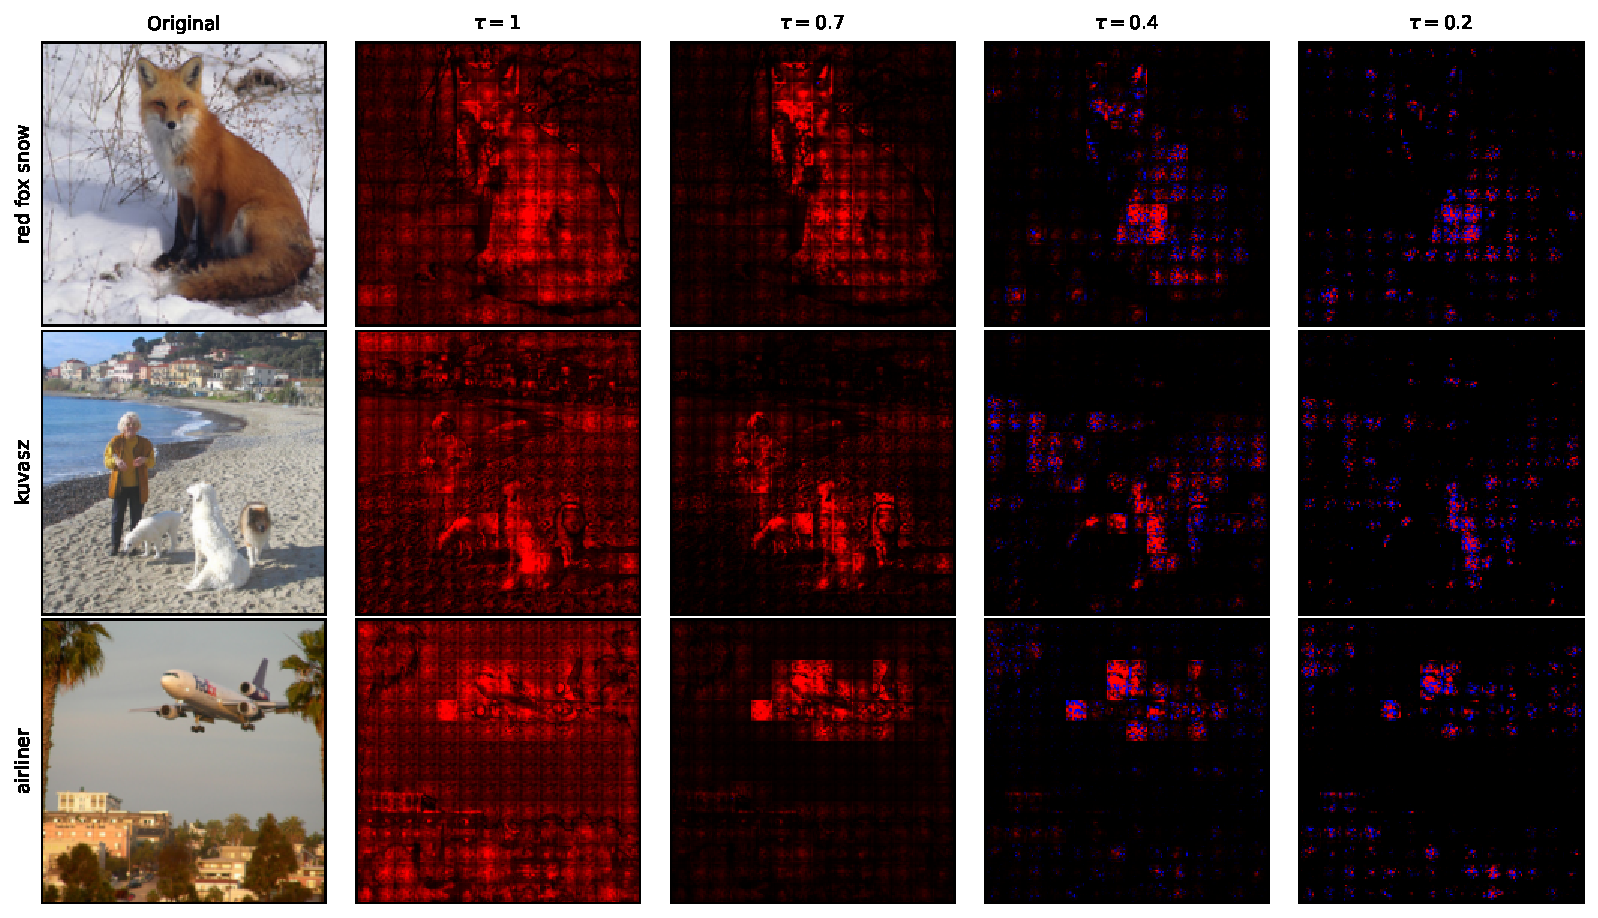
\includegraphics[width=\textwidth]{figures/rg_temperature/rg_temperature_sweep.pdf}
    }
    \caption[Qualitative effect of routing temperature for ViT-B/16]{Temperature controls how strongly backward routing favors larger contributions: in these examples, lowering $\tau$ turns broad heatmaps into sparser maps concentrated on fewer image regions. Routing Game maps on three ImageNet-S examples are shown at $\tau=1,0.7,0.4,0.2$, from left to right. The red fox is from the test split; the kuvasz and airliner are from the validation split. All panels use the same ViT-B/16 checkpoint, target labels, and RG settings ($\alpha=2$, $\beta=1$, $\varepsilon=0.1$, $\lambda_{\mathrm{sm}}=-10$, input variance $5$, merged attention--Value rule); only $\tau$ varies. Each sign is scaled by the image-wise 99th percentile and clipped, with positive relevance in red and negative relevance in blue.}
    \label{fig:vit_temperature}
\end{figure}
